\documentclass{article}
\usepackage[utf8]{inputenc}
\usepackage[T1]{fontenc}
\usepackage[french]{babel}
\usepackage{graphicx}
\usepackage{multicol}
\setlength{\columnsep}{5cm}
\usepackage{hyperref}
\usepackage{textcomp}
\usepackage{gensymb}
\newcommand{\hsp}{\hspace{20pt}}
\newcommand{\HRule}{\rule{\linewidth}{0.5mm}} 
\usepackage{float}
\usepackage{geometry}
\geometry{top=3cm, bottom=3cm, left=3cm, right=3cm}
\usepackage{subcaption}
\usepackage{enumitem}
\usepackage{wrapfig}
\usepackage{algorithm}
\usepackage{algorithmic}
\usepackage{amssymb}
\usepackage{amsmath}
\usepackage{array}




\begin{document}

%%%%%%%%%%%%%%%%%
% PAGE DE GARDE %
%%%%%%%%%%%%%%%%%

\begin{titlepage}
    \begin{sffamily}
        \begin{center}
        
            
\includegraphics[scale=0.2]{../img/Logo_Polytech_Sorbonne.png}\\[1.5cm]
            \textsc{\Large \bfseries{Projet Mathématiques Informatique}}\\[1.5cm]
            % Titre
            \HRule \\[0.4cm]
            { \huge \bfseries Sujet 2\\[0.4cm]}
            \HRule \\[2cm]
            
\includegraphics[scale=0.4]{../img/su.png}\\[2cm]
             % Auteurs
            \begin{minipage}{0.4\textwidth}
                \begin{flushleft} \large
                    \textsc{Tristan MICHEL\\ Kenza EL MHAMDI }
                \end{flushleft}
            \end{minipage}
            \begin{minipage}{0.4\textwidth}
                \begin{flushright} \large
                    \textsc{Aissam RABHI\\ Nael SENOUN    }
                \end{flushright}
            \end{minipage}
            \vfill
        
            % Bas de la page
            {\large 2019-2020}
            
        \end{center}
    \end{sffamily}
\end{titlepage}

%%%%%%%%%%%%
% SOMMAIRE %
%%%%%%%%%%%%

\tableofcontents
\newpage

\setcounter{secnumdepth}{0}
\section{Introduction}
L'objectif du projet est de modéliser ,par le système différentiel ci-dessous, deux espèces en \\compétitions.
\begin{equation}
    (S):
\left\{
\begin{array}{ll}
\frac{dx}{dt} =  x(1 - \frac{x}{k} - \frac{a y}{k}) \\
\frac{dy}{dt} = y(1- \frac{y}{l} - \frac{x^{2}}{l})
\end{array}
\right.
\end{equation}
où x représente le nombre d’individus de la première espèce, y le nombre d’individus de la
deuxième espèce, k est le nombre d’individus de la première espèce que peut nourrir le milieu, l
est le nombre d’individus de la deuxième espèce que peut nourrir le milieu et a est un coefficient.\\Nous allons dans un premier temps réaliser une analyse mathématique du problème. Puis nous le mettrons en oeuvre dans un programme python 

\setcounter{secnumdepth}{1}

\section{Analyse mathématique}

\subsection{Analyse du modèle}
La variation du nombre d'individu d'une espèce dépend de la capacité du milieu à la nourrir (définie par les coefficients k et l). Pour k et l très grands, le terme $(- \frac{x}{k} - \frac{a y}{k})$ sera négligeable, on se retrouve donc avec l'équation
\[\frac{dx}{dt} =x\] \[\frac{dy}{dt} = y\] dont les solutions sont des fonctions exponentielles. \\ On en déduit qu'avec une très grande capacité d'approvisionnement, le nombre d'individu de l'espèce croit de façon exponentielle. \\ Pour un k (ou l) quelconque, la variation du nombre d'individu de l'espèce x (ou y) dépend du signe de  $(1 - \frac{x}{k} - \frac{a y}{k})$ (ou $ (1 -\frac{y}{l} - \frac{x^{2}}{l})$)\\ Pour un instant t fixé, la population augmente a t+dt si :

\begin{equation}
k > x(t) + ay(t) \text{    (ou } l> y(t) + x(t)^{2}) 
\end{equation}
On peut interpréter cette inégalité de la manière suivante :
\begin{itemize}
    \item k et l sont les capacités du milieu à nourrir x et y
    \item x (respectivement y)est le nombre d'individu nourris par le milieu k (resp. l)
    \item a est un coefficient (entre 0 et 1) représentant le pourcentage d'individus de y nourris par le milieu k.
    \item le terme $x + ay$ $(\text{ou } y+ x^{2})$ est la consommation dans k (ou l)
    \item lorsque la consommation dépasse la capacité, il n'y a plus assez de provisions et la population de x (ou de y) diminue
\end{itemize}
Nous allons dans ce projet étudier le comportement du modèle en fonction de différents paramètres, essayer de trouver un équilibre entre deux espèces en compétitions dans un même milieu.
\subsection{Analyse de la stabilité}
Le problème donné est un système non linéaire, on cherche les points singuliers du système en résolvant l'équation $f(x,y) = (0,0) $ avec :
$$
f(x,y) = 
\begin{pmatrix}
x(1 - \frac{x}{k} - \frac{\alpha y}{k}) \\
 y(1- \frac{y}{l} - \frac{x^{2}}{l})
\end{pmatrix}
$$
On a deux équations du second ordre à résoudre : \\ \\
Les solutions de l'équation \[x - \frac{x^{2}}{k} - \frac{ayx}{k} = 0\] sont  $x = 0, x= k- ay$\\
Pour x=0, on a deux solutions de \[y(1- \frac{y}{l}) = 0\] $y= 0$ et $y = l $  \\
Pour y=0, on a deux solutions de \[x - \frac{x^{2}}{k} = 0\]
$x=0$  et  $x=k$
Les points critiques du système sont $(0,0), (k,0), (0,l)$ et $(k-ay,l-x^{2})$ On calcule maintenant les coordonnées de ce dernier points en fonction des paramètres.


$$
\left\{
\begin{array}{ll}
x = k- ay \\
y = l - x^{2}
\end{array}
\right.
$$

$$
 \text{<=>}
\left\{
\begin{array}{ll}
-ax^{2}  +x + (al -k) =0\\
y + x^{2} = l
\end{array}
\right.
$$
Les solutions de la première équation sont :  
$$
x_{1} = \frac{-1 + \sqrt{\Delta}}{2a}  \text{ et } x_{1} = \frac{-1 - \sqrt{\Delta}}{2a}
\text{  avec  }  \Delta = 1 + 4(al -k)\\
$$
Les 2 derniers points critiques du système sont
$$
(k-al -  \frac{1 - \sqrt{ 1 + 4(al -k)}}{2a},l +  (\frac{1 - \sqrt{ 1 + 4(al -k)}}{2a})^{2}) \text{ et } (k-al +  \frac{1 - \sqrt{ 1 + 4(al -k)}}{2a},l +  (\frac{1 + \sqrt{ 1 + 4(al -k)}}{2a})^{2})
$$ 
\\définis seulement pour $\Delta > 0$ soit : $a > \frac{1}{l}(k - \frac{1}{4})$
\section{Mise en oeuvre}
On teste les points critiques comme conditions initiales : \\
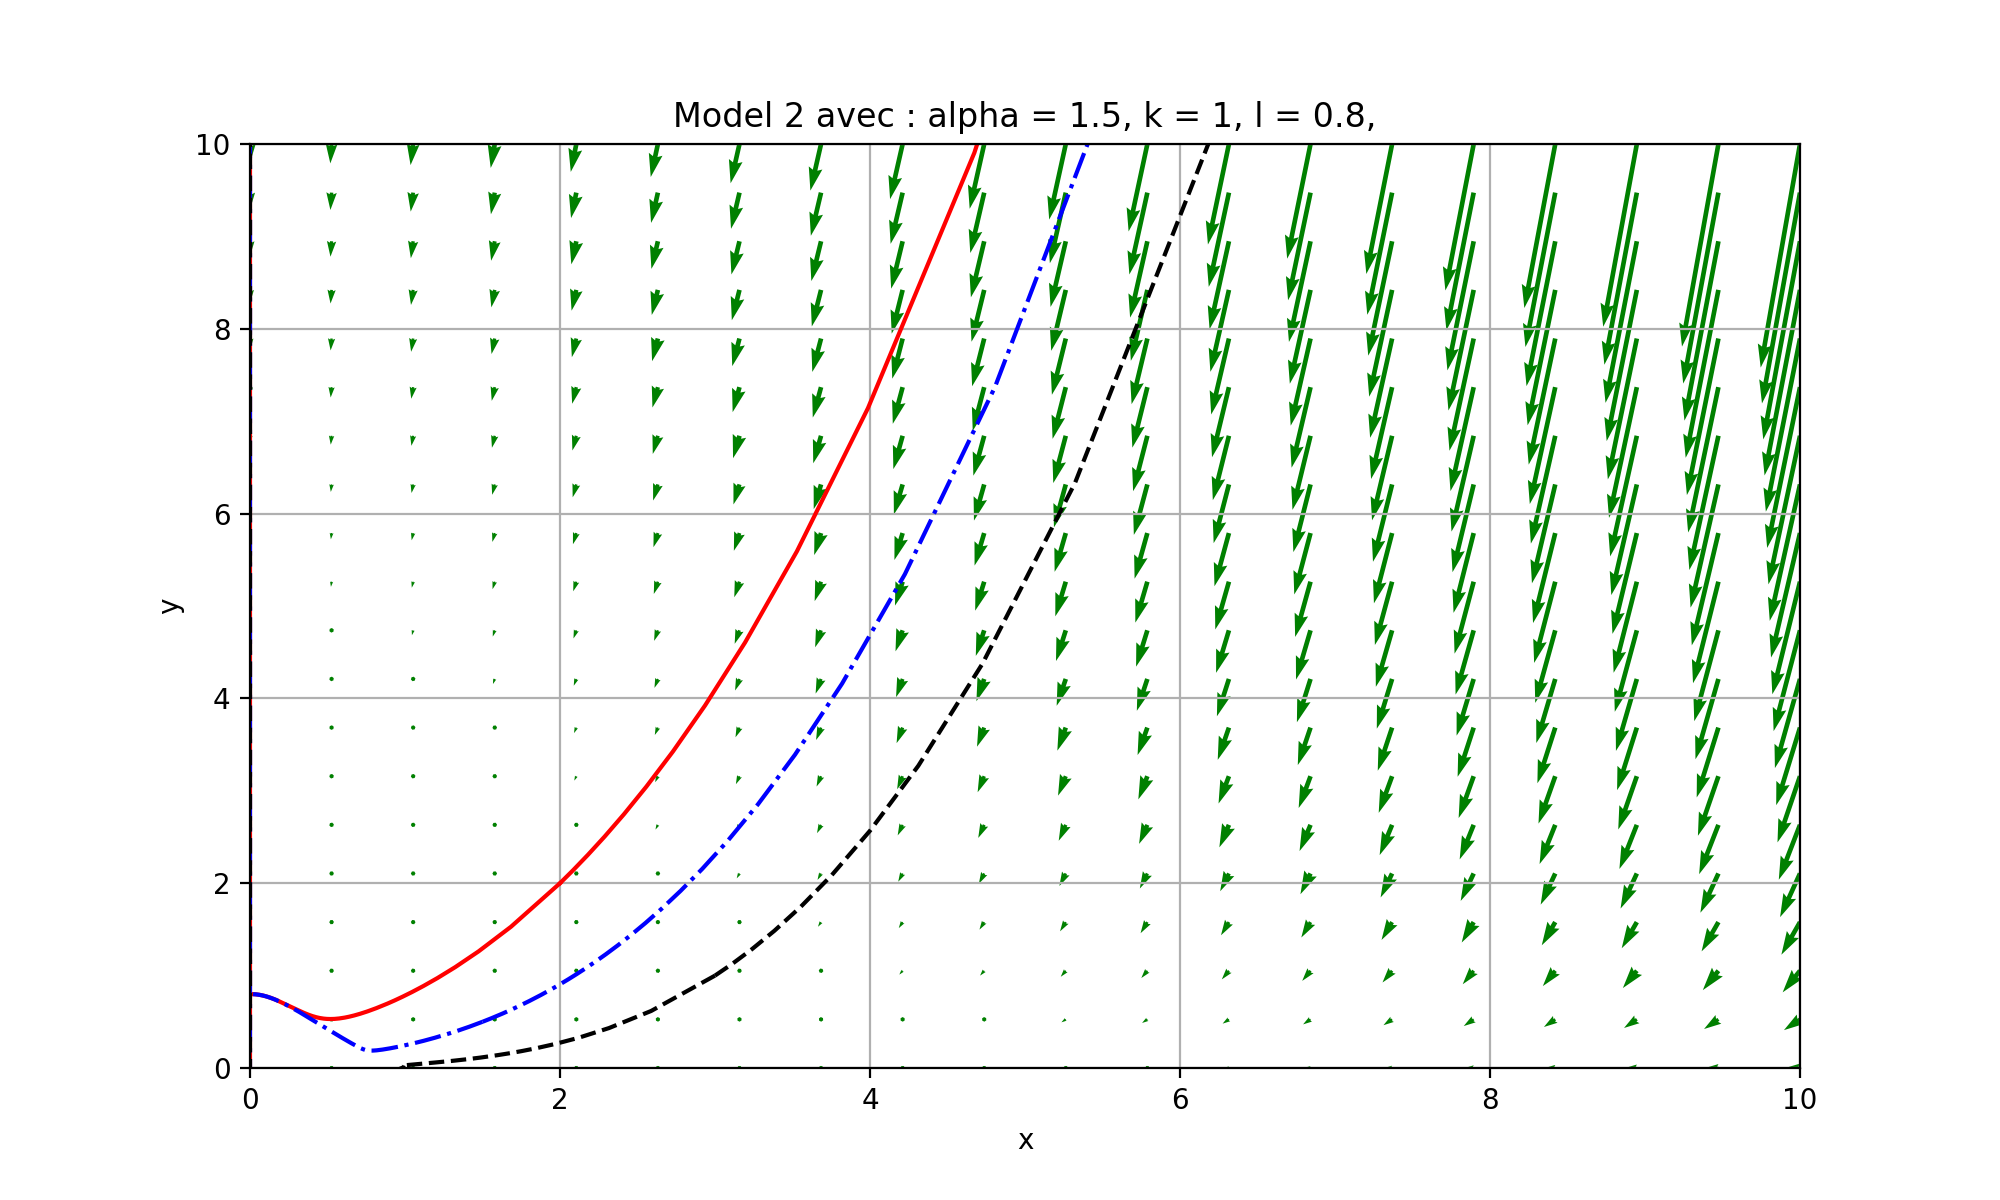
\includegraphics[scale = 0.4]{../../pysrc/img/Model_2.png} \\
On remarque qu'aucune courbe n'est tracée que pour la conditions (1,1) qui n'est pas un point critique.
\end{document}

